\begin{frame}{Git Basics}{Architecture}
  \begin{itemize}
    \item Remote: The central repo (on a host machine/server, e.g., Github or Gitlab)
      {\color{red}$\rightarrow$ is identified by the alias "origin"}
    \item Repository: The local repo (.git sub-directory inside your working directory), created by "git init" or "git clone", i.e., ceartion/clonining
    \item Index or staging area: State between the working directory and repository (after modifying and before commiting)
    \item Workspace or working directory: your local machine, including all directories, sub-directories, and files of your project
  \end{itemize}
  \begin{figure}
    \begin{center}
    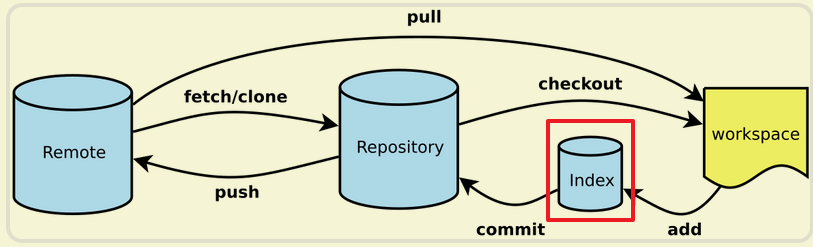
\includegraphics[width=0.8\linewidth]{pics/architecture.png}
    \vspace{-0.3cm}
    \caption{\footnotesize Git architecture (Source: www.stackoverflow.com)}
  \end{center}
\end{figure}

\end{frame}

\begin{frame}{Git Basics}{Definitions}
  \begin{itemize}
    \item \textbf{origin}: A shorthand name for the remote repo
      \comm{git remote show} (shows "origin" as output)
      \comm{git remote show origin} (shows detailed info on origin)
\item \textbf{branch}: A movable pointer to a commit
\item \textbf{master (or sometimes main)}: Default name of the (first) branch: can be changed
\item \textbf{HEAD}: A special pointer that tells on (the tip of) which branch you are.
\item \textbf{origin/HEAD}: A special pointer that tells on which branch the remote repo is.
\end{itemize}
\end{frame}


